\documentclass{article}

\usepackage{fullpage}
\usepackage{nopageno}
\usepackage{amsmath}
\usepackage{amsfonts}
\usepackage{graphicx}
\usepackage{framed}
\usepackage{xcolor}
\usepackage{textcomp}

\definecolor{dark_red}{rgb}{0.5,0.0,0.0}
\definecolor{dark_green}{rgb}{0.0,0.5,0.0}
\definecolor{dark_blue}{rgb}{0.0,0.0,0.5}
\definecolor{blue}{rgb}{0.0,0.0,1.0}

\newcommand{\dr}[1]{\textcolor{dark_red}{#1}}
\newcommand{\dg}[1]{\textcolor{dark_green}{#1}}
\newcommand{\db}[1]{\textcolor{dark_blue}{#1}}
\newcommand{\blue}[1]{\textcolor{blue}{#1}}

\begin{document}


\section{Symbols and quantities}

The essence of algebra revolves around the use of symbols such as the Latin characters \(a\), \(A\), \(b\), \(B\), \(c\), \(C\), \(d\), \(D\) etc. to name both quantities and concepts. Greek letters and other symbols also see use.

As an example, for the current scenario we can define the symbol \(x\) as another name for the number \(5.671\), which is described by the equation \(x = 5.671\). Now whenever the number \(5.671\) appears, it can be replaced with \(x\). For example, 

\(3 \times 5.671^2 - 5.671 + 4 = 3 \times x^2 - x + 4\) 

Also, the multiplication symbol \(\times\) is often omitted for simplicity so the above expression is \(3x^2 - x + 4\).  

Why would one use symbols as ``stand ins" for actual numbers? Below are listed some reasons:

\begin{itemize}
%%%%%%
\item {\bf The number is not yet known.} 
Consider for example the famous equation 
\[E = mc^2\]
where the symbol \(E\) is an object's energy, \(m\) is the object's mass, and \(c\) is the speed of light. While the speed of light \(c \approx 299,\!792,\!458\text{m/s}\) is known, the values of \(m\) and \(E\) are dependent on the object to be considered and are not yet known. Also many physicists use the approximation \(c \approx 300,\!000,\!000\text{m/s}\), and by using the symbol \(c\), the approximation does not have to be chosen immediately. 
%%%%%%
\item {\bf The number's value is not fixed so that the following discussion/formula applies to all cases.}
Referring again to \(E = mc^2\), by not fixing the values of \(m\) and \(E\), the equation applies to all particles instead of particles with a specific mass and energy. It is important to note that not every variable is ``to be solved for". Some variables simply exist to keep the discussion general to all cases and the calculations exact and clean (no approximations).
%%%%%%
\item {\bf The number is too complicated to be repeatedly written in full.} 
Referring again to \(E = mc^2\), the speed of light \(c\) is \(299,\!792,\!458\text{m/s}\) and this is a rather complicated number to write every single time. %To go even further, the Arabic symbols are an abbreviation 
%%%%%%
\item {\bf The symbol indicates the number's meaning.} 
The symbol also conveys the meaning of the number. Within the context of special relativity, the symbol \(c\) is immediately recognized as the speed of light, while the number \(299,\!792,\!458\text{m/s}\) is harder to recognize, especially when multiple approximations are possible. The symbol \(m\) is immediately recognized as representing mass, and \(E\) is immediately recognized as representing energy. {\bf It is important however to recognize that a symbol's meaning will change from scenario to scenario.} Outside of physics, \(c\) may have an entirely different meaning. 
%%%%%%
\item {\bf To simplify a complicated expression/equation.} 
Consider the expression:
\[\frac{5(\pi - 3)(\sqrt{2} + \sqrt{3}) + \frac{1}{\sqrt{2} + \sqrt{3}} + (\pi - 3)^2}{100(\sqrt{2} + \sqrt{3})} + (\pi - 3)\]
By letting \(A = \pi - 3\) and \(B = \sqrt{2} + \sqrt{3}\), the above expression becomes:
\[\frac{5AB + \frac{1}{B} + A^2}{100B} + A\]
which is a much simpler expression to work with or evaluate.
\end{itemize} 

{\bf Not every variable is a quantity to be ``solved for". As indicated above, variables have other uses.}

{\bf From here on out, the multiplication symbol \(\times\) will be replaced in favor of a floating dot \(\cdot\), or be omitted altogether in a manner that does not introduce ambiguity. For example:}

\[2 \times 3  = 2 \cdot 3 = (2)(3) = 6\]

The parenthesis distinguish \((2)(3)\) from the number \(23\). They are not necessary if one factor is a symbol: \((2)(x) = 2x\). 

The division symbol \(\div\) will never appear again, with \(a \div b\) being replaced with \(\frac{a}{b}\) or \(a/b\).

A ``general form" of an expression is an expression that contains placeholder symbols that are to be replaced with other expressions. For example, given the general form \((a + b)(a - b)\), \(a\) and \(b\) are placeholder symbols that can be replaced with specific expressions or numbers. For example, if \(a = 5x\) and \(b = 3\), then the expression \((a + b)(a - b)\) becomes \((5x + 3)(5x - 3)\).





\section{Sets}

Mathematics involves more than just numbers. In the topics that are covered in this class, a basic understanding of the notation related to ``sets" of entities is incredibly useful.  

\begin{itemize}
\item A ``set" is a collection of objects referred to as ``elements". Elements can be, but are not limited to, numbers.
\item Sets {\bf do not} contain duplicate elements.
\item A set will be denoted by listing the elements enclosed by \(\{...\}\). The ordering of the elements does not matter. Duplicate elements are ignored.
\item The empty set is denoted by \(\emptyset\) or \(\{\}\).
\item Sets \(A\) and \(B\) are equal \(A = B\) if and only if \(A\) and \(B\) have the same elements. Every element of set \(A\) can be found in set \(B\) and vice versa.
\item \(x \in A\) if and only if \(x\) belongs to set \(A\). \(x \notin A\) if and only if \(x\) does not belong to set \(A\).
\end{itemize}

\textbf{Examples:}
\begin{itemize}
\item \(\{1, 6, 5\} = \{5, 1, 6\} = \{5, 1, 1, 6\}\)
\item \(2 \in \{4, 2, 3\}\)
\item \(5 \notin \{4, 2, 3\}\)
\end{itemize}

\textbf{Important set of numbers:}
\begin{itemize}
\item ``natural numbers": \(\mathbb{N} = \{1, 2, 3, 4, ...\}\)
\item ``whole numbers": \(\mathbb{W} = \{0, 1, 2, 3, 4, ...\}\)
\item ``integers": \(\mathbb{Z} = \{..., -4, -3, -2, -1, 0, 1, 2, 3, 4, ...\}\)
\item ``rational numbers": \(\mathbb{Q}\) is the set of all numbers that are the division of two integers. 
\item ``real numbers": \(\mathbb{R}\) is the set of all numbers that are distances and their negatives. The set of real numbers contains the set of rational numbers.
\item ``irrational numbers": \(\mathbb{I}\) is the set of all real numbers that are not also rational. % = \mathbb{R} \setminus \mathbb{Q}\)
\end{itemize}

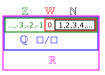
\includegraphics[width = 0.5\textwidth]{set_of_real_numbers}

\textbf{Examples:}

\begin{itemize}
\item Classify \(\sqrt{2}\): Irrational
\item Classify \(-4\): Integer, but not a whole number
\item Classify \(6/3\): Natural number
\item Classify \(0\): Whole number, but not a natural number
\item Classify \(-4/5\): Rational number, but not an integer
\item Classify \(100\): Natural number
\end{itemize}

How can large sets, or sets with an infinite number of elements be denoted? Here will be introduced {\bf set builder notation}. A set can be denoted by the syntax:
\[\{\dr{\text{expression}}|\dr{\text{condition}}\}\]
The ``\(\dr{\text{expression}}\)" is an algebraic expression, most often a single variable, whose attainable values form the elements of the set. The ``\(\dr{\text{condition}}\)" is a condition that must be satisfied for the value of the expression to count towards the set. The symbol ``\(|\)" reads as ``where".
%``Set builder" notation: \(\{x | \text{condition}(x)\}\) or \(\{x : \text{condition}(x)\}\) or \(\{x \in D | \text{condition}(x)\}\) or \(\{x \in D : \text{condition}(x)\}\)
To help denote conditions, the following notations will be used to shorten the description of conditions:

\begin{itemize}
\item Given conditions \(A\) and \(B\), \(A \wedge B\) denotes \(A\) ``AND" \(B\)
\item Given conditions \(A\) and \(B\), \(A \vee B\) denotes \(A\) ``OR" \(B\)
\item Given condition \(A\), \(\neg A\) denotes ``NOT" \(A\)
\item Given conditions \(A\) and \(B\), \(A \implies B\) denotes that the truth of \(A\) ``implies" the truth of \(B\) (\(A\) is true only if \(B\) is also true). This notation is important when solving equations. For example, \(x = 2 \implies x^2 = 4\). Also, \(x \geq 3 \implies x \geq 2\).
\item Given conditions \(A\) and \(B\), \(A \iff B\) denotes that \(A\) is true ``if and only if" (abbreviated by ``iff") \(B\) is true. \(A\) and \(B\) are either both true, or both false. This notation is important when solving equations. For example, \(x + 1 = 3 \iff x = 2\). Also, \(x^2 = 4 \iff ((x = 2) \vee (x = -2))\).
\item Given set \(A\) and condition \(B(x)\) (\(B(x)\) depends on \(x\)), the notation \(\forall x : B(x)\) denotes ``for all values of \(x\), \(B(x)\) is true". The notation \(\forall x \in A : B(x)\) denotes ``for all values of \(x\) from set \(A\), \(B(x)\) is true". For example, \(\forall x \in \mathbb{R} : (x + 1) - 1 = x\).
\item Given set \(A\) and condition \(B(x)\) (\(B(x)\) depends on \(x\)), the notation \(\exists x : B(x)\) denotes ``there exists a value of \(x\) such that \(B(x)\) is true". The notation \(\exists x \in A : B(x)\) denotes ``there exists a value of \(x\) from set \(A\) such that \(B(x)\) is true". For example, \(\exists x \in \mathbb{R} : x + 4 = 10\).
\end{itemize}

\textbf{Examples}
\begin{itemize}
\item The set of rational numbers \(\mathbb{Q}\) can be denoted by \(\mathbb{Q} = \{n/m | (n \in \mathbb{Z}) \wedge (m \in \mathbb{Z})\}\)
\item The set of even integers can be denoted by either \(\{2n | n \in \mathbb{Z}\}\) or by \(\{n | \exists m \in \mathbb{Z} : 2m = n\}\)
\item The set of odd integers can be denoted by either \(\{2n+1 | n \in \mathbb{Z}\}\) or by \(\{n | \neg\exists m \in \mathbb{Z} : 2m = n\}\)
\item The set of square integers can be denoted by either \(\{n^2 | n \in \mathbb{Z}\}\) or by \(\{n | \exists m \in \mathbb{Z} : m^2 = n\}\)
\end{itemize}

In many cases, when the values of the ``\dr{expression}" are to be limited to a set \(A\), the notation:
\[\{\dr{\text{expression}} \in A|\dr{\text{condition}}\}\]
replaces 
\[\{\dr{\text{expression}}| (\dr{\text{expression}} \in A) \wedge \dr{\text{condition}}\}\]




\subsection{Set operators and relations}

\begin{itemize}
\item Sets \(A\) and \(B\) are equal if and only if \(A\) and \(B\) have the same elements: \(\forall x : (x \in A) \iff (x \in B)\)
\item Set \(B\) is a subset of set \(A\), denoted by \(B \subseteq A\), if and only if the elements of \(B\) can also be found in \(A\): \(\forall x : (x \in B) \implies (x \in A)\)
\item Set \(B\) is a proper subset of set \(A\), denoted by \(B \subset A\), if and only if \(B \subseteq A\) and \(B \neq A\)
\item The union of two sets \(A\) and \(B\) is a set that consists of the elements from both sets. Duplicate elements are not included. \(A \cup B = \{x | (x \in A) \vee (x \in B)\}\)
\item The intersection of two sets \(A\) and \(B\) is a set that consists of the elements that are common to both sets. \(A \cap B = \{x | (x \in A) \wedge (x \in B)\}\)
\item The ``set difference" between sets \(A\) and \(B\) consists of all elements of \(A\) that do not also appear in \(B\). \(A \setminus B = \{x | (x \in A) \wedge \neg(x \in B)\}\)
\item The number of unique elements in set \(A\) is denoted by \(|A|\).
\end{itemize}

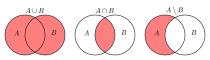
\includegraphics[width = \textwidth]{set_operations}

\textbf{Examples:}
\begin{itemize}
\item \(\{3, 4\} \subset \{4, 2, 3\}\)
\item \(\{3, 4\} \subseteq \{4, 2, 3\}\)
\item \(\{3, 4, 2\} \not\subset \{4, 2, 3\}\)
\item \(\{3, 4, 2\} \subseteq \{4, 2, 3\}\)
\item \(\{1, -1, 3\} \cup \{4, -2\} = \{1, -1, 3, 4, -2\}\)
\item \(\{1, -1, 4\} \cup \{4, -2\} = \{1, -1, 4, -2\}\)
\item \(\{1, -1, 4\} \cap \{4, -2\} = \{4\}\)
\item \(\{1, -1, 3\} \cup \emptyset = \{1, -1, 3\}\)
\item \(\{1, -1, 3\} \cap \emptyset = \emptyset\)
\item \(\{1, -1, 3\} \setminus \{4, -2\} = \{1, -1, 3\}\)
\item \(\{1, -1, 4\} \setminus \{4, -2\} = \{1, -1\}\)
\item \(|\{7, 2, 1\}| = 3\)
\item \(|\{1, 2, 1\}| = 2\)
\item \(|\emptyset| = 0\)
\end{itemize}

In many cases, the set of all real numbers between two bounds \(a\) and \(b\) needs to expressed in a compact manner. For this purpose interval notation is introduced. Given bounds \(a\) and \(b\) where \(a < b\),
\begin{itemize}
\item \((a, b) = \{x \in \mathbb{R} | a < x < b\}\)
\item \((a, b] = \{x \in \mathbb{R} | a < x \leq b\}\)
\item \([a, b) = \{x \in \mathbb{R} | a \leq x < b\}\)
\item \([a, b] = \{x \in \mathbb{R} | a \leq x \leq b\}\)
\end{itemize}





%\section{Algebraic Expressions}  
%
%\begin{itemize}
%\item Contains at least 1 variable.
%	\begin{itemize}
%	\item yes \(5x + 3\)
%	\item no \(5 \cdot 2 + 3\) 
%	\end{itemize}
%\item Is syntactically correct.
%	\begin{itemize}
%	\item yes \((6 + y) \cdot \frac{-3}{y^2 + 2}\)
%	\item no \((6 + y( \cdot \frac{-3}{y^)2 + 2}\)
%	\end{itemize}
%\end{itemize}



\section{Order of Operations}

Algebraic expressions are built up from simpler expressions using mathematical functions. For example, the sum of \(x + 3\) and \(2y\) is \((x + 3) + 2y\), where \(x + 3\) and \(2y\) are ``subexpressions". As expressions get large, the grouping of terms into sub expressions become ambiguous.

Operator precedence:
\[(\Box) \succ  \Box^\Box \succ \times,/,\div \succ +,-\] 
For operators of equal precedence, grouping occurs from left to right. 

\begin{itemize}
%%%%%%%%%%%%%
\item 
\begin{tabular}{cc}
\(5 \cdot 3 - 4 = (5 \cdot 3) - 4 = 15 - 4 = 11\) & \(5 \cdot (3 - 4) = 5 \cdot (-1) = -5\) \\

\includegraphics[scale = 0.8]{expression_tree_1} & 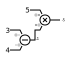
\includegraphics[scale = 0.8]{expression_tree_2} 
\end{tabular}
%%%%%%%%%%%%%
\item 
\begin{tabular}{cc}
\(2 \cdot 3^2 - 4 = (2 \cdot (3^2)) - 4 = 2 \cdot 9 - 4 = 18 - 4 = 14\) & \((2 \cdot 3)^2 - 4 = 6^2 - 4 = 36 - 4 = 32\) \\
\includegraphics[scale = 0.8]{expression_tree_3} & 
\includegraphics[scale = 0.8]{expression_tree_4}
\end{tabular}
%%%%%%%%%%%%%
\item 
\begin{tabular}{cc}
\(6 - 7 + 5 = -1 + 5 = 4\) & \(6 - (7 + 5) = 6 - 12 = -6\) \\ 

\includegraphics[scale = 0.8]{expression_tree_5} & \includegraphics[scale = 0.8]{expression_tree_6}
\end{tabular}
%%%%%%%%%%%%%
\item 
\begin{tabular}{cc}
\(3 / 4 \cdot 5 = \frac{3}{4} \cdot 5 = \frac{15}{4}\) & \(3 / (4 \cdot 5) = 3 / 20 = \frac{3}{20}\) \\ 

\includegraphics[scale = 0.8]{expression_tree_7} & 
\includegraphics[scale = 0.8]{expression_tree_8}
\end{tabular}
%%%%%%%%%%%%%
%\item 
%\begin{tabular}{cc}
%\(x - y + z = x + (-y) + z\) & \(x - (y + z) = x + (-y) + (-z)\) \\ 
%
\includegraphics[scale = 0.8]{expression_tree_9} & \includegraphics[scale = 0.8]{expression_tree_10}
%\end{tabular}
\end{itemize}

{\bf Any time a minus (\(-\)) sign is encountered, it should be always be interpreted as the addition of the right hand quantities' negative:}

\begin{itemize}
\item \[x - y = x + (-y)\]

\includegraphics[scale = 0.8]{expression_tree_11} 
\item \[x - y + z = x + (-y) + z \quad\text{not}\quad x - (y + z)\]

\includegraphics[scale = 0.8]{expression_tree_12}
\item \[-b + 4a - c - 3d = (-b) + (4a) + (-c) + (-3d)\]
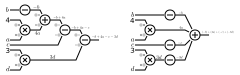
\includegraphics[scale = 0.65]{expression_tree_13}
\end{itemize}




%\section{Substitution}
%
%\begin{itemize}
%\item \(x = 2\) and \(y = \frac{2x + 3}{x - 1}\) implies that \(y = \frac{2(2) + 3}{2 - 1} = \frac{4 + 3}{1} = 7\)
%\item \(x = 3\) and \(y = x^x - 7\) implies that \(y = 3^3 - 7 = 27 - 7 = 20\)
%\item \(x = -4\); \(y = 5\); and \(z = 5x + 3y\) implies that \(z = 5(-4) + 3(5) = -20 + 15 = -5\)
%\end{itemize}



\section{Division}

The division of a number \(a\) by \(b\), originally denoted by \(a \div b\), but almost always by \(a/b\) or \(\frac{a}{b}\), has somewhat different, but ultimately equivalent, understandings:
\begin{itemize}
\item \textbf{Understanding 1:} When \(a\) is evenly divided into \(b\) pieces, the {\bf quotient} \(a/b\) is the amount of each piece. For example, \(1/4\) is \(1\) evenly divided into \(4\) pieces.
\item \textbf{Understanding 2:} The {\bf quotient} \(a/b\) is the number of copies of \(b\) that are needed to be summed together to get \(a\). For example, \(1/4\) is the number (albeit fractional) of copies of \(4\) needed to total to \(1\). 
\end{itemize}
Borrowing the terminology from fractions, \(a\) will be referred to as the numerator, and \(b\) will be referred to as the denominator.

The two understandings of division is similar to the fact that there are two understandings of the product \(a \times b\). The product can be viewed as either the sum of \(b\) copies of \(a\), or the sum of \(a\) copies of \(b\). The analogy is shown in the image below. In the lower diagrams, the product \(a \times b\) is \(b\) copies of \(a\), and the quotient \(a/b\) is the equal splitting of \(a\) into \(b\) pieces. In the upper diagrams, the product \(a \times b\) is \(a\) copies of \(b\), and the quotient is the number of copies of \(b\) that need to be summed to get \(a\).

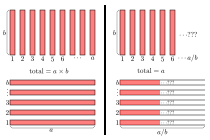
\includegraphics[width = \textwidth]{multiplication_vs_division}



\section{Arithmetic involving fractions}

Here will be a review of arithmetic involving rational numbers, a.k.a. fractions. A rational number has the form \(\frac{a}{b}\) where \(a\) and \(b\) are integers. \(\frac{a}{b}\) is \(a\) copies of \(\frac{1}{b}\), and \(\frac{1}{b}\) is \(1\) divided into \(b\) equal pieces.


\subsection{Multiplication}

Start with two whole numbers \(m\) and \(n\). \(\frac{1}{m}\) is \(1\) divided into \(m\) equal pieces. To multiply any number \(x\) by \(\frac{1}{n}\) is to divide \(x\) into \(n\) equal pieces. Multiplying \(\frac{1}{m}\) by \(\frac{1}{n}\) is to further divide \(\frac{1}{m}\) into \(n\) equal pieces, resulting in \(mn\) pieces of \(1\). Hence:
\[\frac{1}{m} \cdot \frac{1}{n} = \frac{1}{mn}\]

Given rational numbers \(\frac{a}{b}\) and \(\frac{c}{d}\), the product is \(ac\) copies of \(\frac{1}{bd}\):
\[\frac{a}{b} \cdot \frac{c}{d} = \frac{ac}{bd}\] 
The multiplication of two fractions is done by separately multiplying the numerators and the denominators.


\begin{tabular}{cc}
\parbox{0.5\textwidth}{
A \(1 \times 1\) box is shown of the right. This box has an area of \(1\). The horizontal dimension is divided into \(6\) equal pieces. The vertical dimension is divided into \(9\) equal pieces. The area is divided into \(6 \cdot 9 = 54\) small rectangles. The dimensions of each small rectangle are \(\frac{1}{6}\) horizontal by \(\frac{1}{9}\) vertical. The area of one of the small rectangles is \(\frac{1}{6} \cdot \frac{1}{9} = \frac{1}{54}\). The shaded rectangle has dimensions \(\frac{5}{6}\) horizontal by \(\frac{4}{9}\) vertical. The shaded rectangle includes \(5 \cdot 4 = 20\) small rectangles, and has an area of \(\frac{5}{6} \cdot \frac{4}{9} = \frac{20}{54}\).
} & \parbox{0.5\textwidth}{
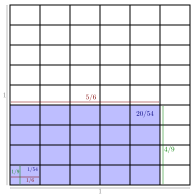
\includegraphics[width = 0.5\textwidth]{multiplying_fractions}
}
\end{tabular}


\subsection{Division}

Given an arbitrary natural number \(n\), dividing \(x\) by \(n\) is to split \(x\) into \(n\) equal parts. Now dividing by the fraction \(\frac{1}{n}\), what does it mean to split \(x\) into \(\frac{1}{n}\) equal parts? To address this confusion, the \(2^\text{nd}\) understanding of division is used. The number of copies of \(\frac{1}{n}\) that need to be summed to get \(1\) is \(n\), so the number of copies of \(\frac{1}{n}\) that need to summed to get \(x\) is \(n x\). Therefore dividing by \(\frac{1}{n}\) is equivalent to multiplying by \(n\). For all numbers \(x\), \(\frac{x}{1/n} = nx\). 

Consider an arbitrary fraction \(\frac{a}{b}\), and an arbitrary number \(x\). \(\frac{a}{b}\) is the product of \(a\) and \(\frac{1}{b}\). Dividing \(x\) by \(\frac{a}{b}\) is done by first dividing \(x\) into \(a\) equal parts, followed by dividing \(\frac{x}{a}\) into ``\(\frac{1}{b}\)" equal parts. However, as previously mentioned, dividing a number into ``\(1/b\)" equal parts is equivalent to multiplication by \(b\). Putting everything together, \(x\) is first divided by \(a\), and then multiplied by \(b\): 
\[\frac{x}{a/b} = \frac{x}{a} \cdot b = x \cdot \frac{b}{a}\]   
Division by \(\frac{a}{b}\) is equivalent to multiplication by the ``reciprocal" \(\frac{b}{a}\).

Given rational numbers \(\frac{a}{b}\) and \(\frac{c}{d}\), the quotient is 
\[\frac{a}{b} \Big/ \frac{c}{d} = \frac{a}{b} \cdot \frac{d}{c}\]


\subsection{Lowest Terms}

Given whole numbers \(a\) and \(b\), the fraction \(\frac{a}{b}\) is \(a\) copies of \(\frac{1}{b}\). \(\frac{1}{b}\) is \(1\) divided into \(b\) equal pieces. Further breaking each copy of \(\frac{1}{b}\) into \(k\) pieces results in \(\frac{a}{b}\) becoming \(ka\) copies of \(\frac{1}{kb}\). The multiplication of the numerator and denominator of a fraction by the same value does not change its value: \(\frac{a}{b} = \frac{k a}{k b}\). Conversely, dividing the numerator and denominator by the same value does not change its value: \(\frac{k a}{k b} = \frac{a}{b}\). When the numerator and denominator of a fraction have a common factor, the common factor can be removed from both the numerator and denominator. 

Consider the fraction: 
\[\frac{6}{15}\] 
both the numerator and denominator have \(3\) as a common factor. Since \(\frac{1}{15}\) is \(\frac{1}{5}\) broken into \(3\) pieces, \(\frac{3}{15} = \frac{1}{5}\). \(\frac{6}{15}\) is \(2\) copies of \(\frac{3}{15}\) so \(\frac{6}{15} = 2 \cdot \frac{3}{15} = 2 \cdot \frac{1}{5} = \frac{2}{5}\). The factor of \(3\) has been eliminated from the numerator and the denominator.

The elimination of all factors that are common to both the numerator and denominator is referred to as reducing a fraction to its lowest terms. This can be done by fully factorizing the numerator and denominator into a product of prime numbers, and eliminating the common factors:

\begin{itemize}
\item \[\frac{108}{36} = \frac{2 \cdot 2 \cdot 3 \cdot 3 \cdot 3}{2 \cdot 2 \cdot 3 \cdot 3} = \frac{\not{2} \;\cdot \not{2} \;\cdot \not{3} \;\cdot \not{3} \cdot 3}{\not{2} \;\cdot \not{2} \;\cdot \not{3} \;\cdot \not{3}} = \frac{3}{1} = 3\]
\item \[\frac{45}{27} = \frac{3 \cdot 3 \cdot 5}{3 \cdot 3 \cdot 3} = \frac{\not{3} \;\cdot \not{3} \;\cdot 5}{\not{3} \;\cdot \not{3} \;\cdot 3} = \frac{5}{3}\]
\item \[\frac{-60}{105} = -\frac{2 \cdot 2 \cdot 3 \cdot 5}{3 \cdot 5 \cdot 7} = -\frac{2 \cdot 2 \;\cdot \not{3} \;\cdot \not{5}}{\not{3} \;\cdot \not{5} \;\cdot 7} = -\frac{4}{7}\]
\end{itemize}



\subsection{Addition}

Adding fractions (rational numbers) where the denominators are equivalent is a trivial matter. Consider the sum:

\[\frac{7}{5} + \frac{4}{5}\]

The sum involves \(7\) copies of \(\frac{1}{5}\) and \(4\) copies of \(\frac{1}{5}\). The total is \(7 + 4 = 11\) copies of \(\frac{1}{5}\), for a total of \(\frac{11}{5}\):

\[\frac{7}{5} + \frac{4}{5} = 7(\frac{1}{5}) + 4(\frac{1}{5}) = 11(\frac{1}{5}) = \frac{11}{5}\]


When the denominators are not equal, the sum involves unequal units. As an example of adding unequal units, consider the problem adding coins with different denominations. 
\begin{itemize}
\item \(1 \; \text{quarter} = 25\text{\textcent} = 0.25\$\) 
\item \(1 \; \text{dime} = 10\text{\textcent} = 0.1\$\)
\item \(1 \; \text{nickel} = 5\text{\textcent} = 0.05\$\) 
\end{itemize}

When adding \(3 \; \text{quarters}\) to \(5 \; \text{dimes}\), both units of currency need to be broken down into whole numbers of a common unit of currency. A quarter is \(5 \; \text{nickels}\), and a dime is \(2 \; \text{nickels}\), therefore both parts of the sum are whole numbers of nickels which are then easily added together. 

\[3 \; \text{quarters} + 5 \; \text{dimes} = 3 (5 \; \text{nickels}) + 5 (2 \; \text{nickels}) = 15 \; \text{nickels} + 10 \; \text{nickels} = 25 \; \text{nickels}\]

Quarters and dimes are also whole numbers of pennies. A quarter is \(25\text{\textcent}\), and a dime is \(10\text{\textcent}\).

\[3 \; \text{quarters} + 5 \; \text{dimes} = 3 (25\text{\textcent}) + 5 (10\text{\textcent}) = 75\text{\textcent} + 50\text{\textcent} = 125\text{\textcent}\]


How can this be used to add fractions with unequal denominators? Given \(\frac{1}{m}\) and \(\frac{1}{n}\) where \(m\) and \(n\) are whole numbers, by splitting \(\frac{1}{m}\) into \(n\) equal pieces, and \(\frac{1}{n}\) into \(m\) equal pieces, we get the common value of \(\frac{1}{mn}\). \(mn\) is referred to as a common denominator. It can now be observed that \(\frac{1}{m}\) is \(n\) copies of \(\frac{1}{mn}\), and \(\frac{1}{n}\) is \(m\) copies of \(\frac{1}{mn}\).

As an example, consider the sum:

\[\frac{5}{3} + \frac{7}{4}\]

By splitting \(\frac{1}{3}\) into \(4\) equal pieces, and \(\frac{1}{4}\) into \(3\) equal pieces, we get that \(\frac{1}{3}\) is \(4\) copies of \(\frac{1}{12}\) and that \(\frac{1}{4}\) is \(3\) copies of \(\frac{1}{12}\). Hence \(\frac{1}{3}\) can be replaced with \(\frac{4}{12}\), and \(\frac{1}{4}\) can be replaced with \(\frac{3}{12}\). The sum can be completed as follows: 

\[\frac{5}{3} + \frac{7}{4} = 5(\frac{1}{3}) + 7(\frac{1}{4}) = 5(\frac{4}{12}) + 7(\frac{3}{12}) = \frac{20}{12} + \frac{21}{12} = \frac{41}{12} \quad\dr{( = 3 + \frac{5}{12})}\]

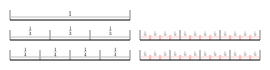
\includegraphics[width = \textwidth]{adding_fractions}


In addition, given \(\frac{1}{m}\) and \(\frac{1}{n}\) where \(m\) and \(n\) are whole numbers, it is not always necessary to split \(\frac{1}{m}\) into \(n\) pieces and \(\frac{1}{n}\) into \(m\) pieces. Let \(p\) denote the ``lowest common multiple" of \(m\) and \(n\). A common multiple of \(m\) and \(n\) is a number that is a multiple of both \(m\) and \(n\). While \(mn\) is a common multiple of \(m\) and \(n\), \(mn\) is not necessarily the lowest common multiple of \(m\) and \(n\). Consider for instance \(m = 4\) and \(n = 6\). \(mn = 24\) is a common multiple of \(m\) and \(n\), but \(p = 12\) is the lowest common multiple of \(m\) and \(n\). If \(p\) is \(a\) times \(m\), then \(\frac{1}{m}\) can be broken into \(a\) pieces of size \(\frac{1}{am} = \frac{1}{p}\). If \(p\) is \(b\) times \(n\), then \(\frac{1}{n}\) can be broken into \(b\) pieces of size \(\frac{1}{bn} = \frac{1}{p}\). \(\frac{1}{m}\) and \(\frac{1}{n}\) are both a whole number of copies of \(\frac{1}{p}\). 

As an example, consider the sum:

\[\frac{3}{4} + \frac{5}{6}\]

The lowest common multiple of \(m = 4\) and \(n = 6\) is \(p = 12\). \(p = 12\) is \(a = 3\) times \(m = 4\), and is \(b = 2\) times \(n = 6\). \(\frac{1}{4}\) is \(3\) copies of \(\frac{1}{12}\), so \(\frac{1}{4} = \frac{3}{12}\). \(\frac{1}{6}\) is \(2\) copies of \(\frac{1}{12}\), so \(\frac{1}{6} = \frac{2}{12}\). The sum can be completed as follows: 

\[\frac{3}{4} + \frac{5}{6} = 3(\frac{1}{4}) + 5(\frac{1}{6}) = 3(\frac{3}{12}) + 5(\frac{2}{12}) = \frac{9}{12} + \frac{10}{12} = \frac{19}{12} \quad \dr{( = 1 + \frac{7}{12})}\]


Given the sum 

\[\frac{5}{2} - \frac{11}{6}\]

The lowest common denominator is \(6\), so the sum is:

\[\frac{5}{2} - \frac{11}{6} = 5(\frac{1}{2}) - 11(\frac{1}{6}) = 5(\frac{3}{6}) - 11(\frac{1}{6}) = \frac{15}{6} - \frac{11}{6} = \frac{4}{6}\]

Since the denominator is a multiple \(2\), and the numerator is also a multiple of \(2\), \(2\) copies of \(\frac{1}{6}\) can be clumped together to get \(\frac{2}{6} = \frac{1}{3}\). The sum can be simplified as follows:
\[\frac{4}{6} = 2(\frac{2}{6}) = 2(\frac{1}{3}) = \frac{2}{3}\]

This is reducing a fraction to ``lowest terms".



Given algebraic expressions, a common multiple is the product of the denominators:

\[\frac{a}{b} + \frac{c}{d} = a(\frac{1}{b}) + c(\frac{1}{d}) = a(\frac{d}{bd}) + c(\frac{b}{bd}) = \frac{ad}{bd} + \frac{bc}{bd} = \frac{ad + bc}{bd}\]





\section{Absolute Value}

The absolute value of a number \(x\) is \(x\) with its sign removed. The absolute value is denoted by \(|x|\). The absolute value describes the ``raw size" of the number.

\[|x| = \left\{\begin{array}{cc} x & (x \geq 0) \\ -x & (x < 0) \end{array}\right.\]

\textbf{Examples:}
\begin{itemize}
\item \(|-6| = 6\)
\item \(|0| = 0\)
\item \(|5.67| = 5.67\)
\item \(|-\pi| = \pi\)
\end{itemize}



\section{Scientific Notation}

With the operations \(+\), \(-\), \(\times\), and especially with \(\div\) and rational numbers, the values attained with successive operations become incrementally more complex. Most rational numbers use an infinite number of decimal places when expressed in decimal form:
\[\frac{1}{3} = 0.33333333333333333333\dots\]

%The expression 
%\[\frac{11 \cdot 9 \cdot 7 \cdot 5 \cdot 3 \cdot 1}{10 \cdot 8 \cdot 6 \cdot 4 \cdot 2}\]
%
%evaluates to
%
%\[\frac{10395}{3840}\]

Below, the product of two 5 digit numbers is shown: 

\[78123 \times 98650 = 7706833950\]

With a single multiplication step, the number of digits in a single number has doubled. Further arithmetic will add even more layers of complexity. Many calculators can't take more than 10 digits. To curtail this complexity, approximations are necessary. 

Quantities measured in the physical world, whether they be time, space, mass, etc., will \emph{always} have some amount of error. When approximations are made, some information will be left behind. The question is which information to keep, and which to discard. This leads to the notion of ``significant digits" and scientific notation. 

The first aspect of a number to keep track of is whether the number is positive or negative.

The next most important property of a number is its raw size. Is the absolute value of the number on a scale similar to \(1\), \(10\), \(100\), \(1000\), etc.? Or perhaps the size is similar to \(0.1\), \(0.01\), \(0.001\), \(0.0001\), etc. If \(n\) is an arbitrary integer, the notation \(10^n\) denotes a \(1\) followed by \(n\) zeros if \(n\) is nonnegative, or if \(n\) is negative, a decimal point followed by \(|n|-1\) zeros with a \(1\) in the \(|n|^{\text{th}}\) decimal place:
\begin{itemize}
\item ...
\item \(10^4 = 10,\!000\)
\item \(10^3 = 1,\!000\)
\item \(10^2 = 100\)
\item \(10^1 = 10\)
\item \(10^0 = 1\)
\item \(10^{-1} = 0.1\)
\item \(10^{-2} = 0.01\)
\item \(10^{-3} = 0.001\)
\item \(10^{-4} = 0.0001\)
\item ...
\end{itemize}

The absolute value of an arbitrary number \(x\) can fall into one of the following infinite number of disjoint intervals:
\begin{itemize}
\item ...
\item \(10^{-4} \leq |x| < 10^{-3}\)
\item \(10^{-3} \leq |x| < 10^{-2}\)
\item \(10^{-2} \leq |x| < 10^{-1}\)
\item \(10^{-1} \leq |x| < 10^0\)
\item \(10^0 \leq |x| < 10^1\)
\item \(10^1 \leq |x| < 10^2\)
\item \(10^2 \leq |x| < 10^3\)
\item \(10^3 \leq |x| < 10^4\)
\item \(10^4 \leq |x| < 10^5\)
\item ...
\end{itemize}

The last piece of information if a multiplier coefficient \(a\), referred to the ``mantissa" that adjusts the value of \(10^n\) to the actual value. \(a\) is in the range \(1 \leq a < 10\), and multiplying \(10^n\) by \(a\) yields a number from the range \(10^n \leq |x| < 10^{n+1}\). It is in the value of \(a\) that accuracy may be discarded, starting with the least significant digits (the right most decimal digits). The most significant digits of \(a\) are the most important parts of \(a\). When approximations are being made, the number of digits of \(a\), referred to as the number of significant digits, that are retained is decided upon. 

In summary, to express a number \(x\) in scientific notation, the following steps are used: 

\begin{itemize}
\item Record the sign of \(x\), and then remove the sign from \(x\).
\item Shift the decimal point of \(x\) left or right until all digits left of the \(1\)'s digit are \(0\), and the \(1\)'s digit is nonzero. The number of leftwards shifts is \(n\). Rightwards shifts make \(n\) negative. \(n\) is the unique integer where the absolute value of \(x\) falls in the interval \(10^n \leq |x| < 10^{n+1}\).  
\item After shifting the decimal point, the remaining number is now the mantissa \(a\). Round \(a\) to the desired number of significant digits.
\item The number \(x\) in scientific notation has the form 
\[x = \pm a \times 10^n\]
where the \(\pm\) is the sign of \(x\).
\end{itemize}  
Lastly, it should be noted that \(0\) in scientific notation is simply \(0\). Other forms for the scientific notation are \(\pm a \text{E} n\) and \(\pm a \text{e} n\). The \(\text{E}\) or \(\text{e}\) do not represent values, and are part of the notation.

%\begin{itemize}
%\item For positive numbers: \(a \times 10^n\) where \(1 \leq a < 10\) and \(n \in \mathbb{Z}\)
%\item For negative numbers: \(-a \times 10^n\) where \(1 \leq a < 10\) and \(n \in \mathbb{Z}\)
%\item \(0\) is simply \(0\)
%\end{itemize}

\textbf{Examples:} \\
\(3\) significant digits will be used: 
\begin{itemize}
\item \(35,\!640,\!000 = 3.56 \times 10^7\) = 3.56E7 = 3.56e7
\item \(5 = 5.00 \times 10^0 = 5.00\text{E}0 = 5.00\text{e}0\)
\item \(-0.234 = -2.34 \times 10^{-1}\) = -2.34E-1 = -2.34e-1
\item \(0 = 0\)
\item \(-10,000,000 = -1.00 \times 10^7\) = -1.00E7 = -1.00e7
\item \(0.0000065 = 6.50 \times 10^{-6}\) = 6.50E-6 = 6.50e-6
\item \(602,000,000,000,000,000,000,000 = 6.02 \times 10^{23}\) = 6.02E23 = 6.02e23
\item \(23.45 \approx 2.35 \times 10^1\) = 2.35E1 = 2.35e1
\item \(346.88 \approx 3.47 \times 10^2\) = 3.47E2 = 3.47e2
\item \(0.02 = 2.00 \times 10^{-2}\) = 2.00E-2 = 2.00e-2
\end{itemize}




\section{Ratios}

A ratio is the ``proportion" between two quantities. Symbolically, a ratio is denoted by the notation 
\[a : b\]
where each group of \(a\) units of quantity 1 corresponds to \(b\) units of quantity 2. The notation reads as ``the ratio of \(a\) to \(b\)".

Ratios are unchanged by multiplying or dividing both sides by the same number:
\[a : b \;\;=\;\; ka : kb \;\;=\;\; a/k : b/k\]
no matter the value of \(k\). All that matters are the {\bf proportions} of the two sides.

Ratios are often quantified by the left hand side value when the right hand side value is \(1\). Dividing both sides of the ratio \(a : b\) by \(b\) yields 
\[a : b \;\;=\;\; a/b : b/b \;\;=\;\; a/b : 1\]
The ratio is often referenced by the quantity \(a/b\), which is the amount of quantity 1 {\bf per} unit of quantity 2. If \(a\) is distance, and \(b\) is time, then the ratio of distance to time is the speed.

\vspace{5mm}

\textbf{Example 1:}

Envision a scenario where a car, {\bf traveling at a constant speed} travels \(40\text{km}\) in \(3\) hours. The ratio of distance traveled to time is:

\[40\text{km} : 3\text{hr}\]   

The following ratios are all equivalent:

\begin{align*}
40\text{km} : 3\text{hr} 
& \;\;=\;\; 80\text{km} : 6\text{hr} 
\;\;=\;\; 120\text{km} : 9\text{hr} 
\;\;=\;\; 160\text{km} : 12\text{hr} 
\;\;=\;\; 60\text{km} : 4.5\text{hr} \\
& \;\;=\;\; 20\text{km} : 1.5\text{hr} 
\;\;=\;\; 10\text{km} : 0.75\text{hr} 
\end{align*}

For each representation of the ratio, the distance listed on the left is the distance traveled by the car in the time listed on the right. In \(9\text{hr}\) for example, the car has traveled \(120\text{km}\).  

Ratios are often quantified by the left hand side value when the right hand side value is \(1\). In the current scenario, the ratio is quantified by the car's speed. The car's speed is determined by the distance traveled in \(1\text{hr}\), and to find this speed, all that is needed is to split the distance of \(40\text{km}\) evenly across the \(3\) hours:

 \[40\text{km} : 3\text{hr} \;\; = \;\; \frac{40\text{km}}{3\text{hr}} : \frac{3\text{hr}}{3\text{hr}} \;\; = \;\; \frac{40}{3}\text{km/hr} : 1\] 

The car's speed is \(v = \frac{40}{3}\text{km/hr}\). In a time span of \(t = 2\text{hr}\), the distance \(d\) traveled by the car is the total sum of a copy of \(v\) for each hour (speed multiplied by time): \(d = t \times v = \frac{80}{3}\text{km}\). 

Given a distance \(d = 15\text{km}\), the time required to travel this distance is the number of copies of \(v\) that need to be summed to get \(d\): \(t = \frac{d}{v} = \frac{15}{40/3}\text{hr} = \frac{45}{40}\text{hr} = \frac{9}{8}\text{hr}\) 

\vspace{5mm}

\textbf{Example 2:}

Now consider another scenario. \(7.123\text{L}\) of a mysterious liquid has a mass of \(3.458\text{kg}\). How much volume of the liquid is present when the mass is \(46.55\text{kg}\)? The volume to mass ratio is:
\[7.123\text{L} : 3.458\text{kg}\]

There are two approaches to finding the volume associated with a mass of \(46.55\text{kg}\). 

\textbf{Approach 1:}

The volume of each unit of mass is \(\frac{7.123\text{L}}{3.458\text{kg}} \approx 2.060\text{L/kg}\) (The \(1^\text{st}\) understanding of division is used.). With the desired mass being \(46.55\text{kg}\), the total volume is \(46.55\text{kg} \times 2.060\text{L/kg} \approx 95.89\text{L}\).

\textbf{Approach 2:}

The number of copies of \(3.458\text{kg}\) present in \(46.55\text{kg}\) is \(\frac{46.55\text{kg}}{3.458\text{kg}} \approx 13.46\) (The \(2^\text{nd}\) understanding of division is used.). Converting each copy of \(3.458\text{kg}\) to the corresponding \(7.123\text{L}\), the total volume is \(13.46 \times 7.123\text{L} \approx 95.88\text{L}\).

\vspace{5mm}

\textbf{Example 3:}

A mass of \(24.78\text{kg}\) of an unknown metal has a volume of \(2.413\text{L}\), and costs \(\$164.20\). 
\begin{itemize}
\item What is the mass of \(15.00\text{L}\) of this metal? 
\item How much of this metal, in terms of mass, can be purchased with \(\$30.00\)? 
\end{itemize}

Addressing the first question, the mass to volume ratio is 
\[24.78\text{kg} : 2.413\text{L}\]

The amount of mass per unit volume (1L) is \(\frac{24.78\text{kg}}{2.413\text{L}} \approx 10.27\text{kg/L}\) (The \(1^\text{st}\) understanding of division is used.). With the desired volume being \(15.00\text{L}\), the total mass is \(15.00\text{L} \times 10.27\text{kg/L} \approx 154.1\text{kg}\)

Alternately, the number of copies of \(2.413\text{L}\) present in \(15.00\text{L}\) is \(\frac{15.00\text{L}}{2.413\text{L}} \approx 6.216\) (The \(2^\text{nd}\) understanding of division is used.). Converting each copy of \(2.413\text{L}\) to the corresponding \(24.78\text{kg}\), the total mass is \(6.216 \times 24.78\text{kg} \approx 154.0\text{kg}\)

Addressing the second question, the mass to cost ratio is
\[24.78\text{kg} : \$164.20\]

The amount of mass per dollar is \(\frac{24.78\text{kg}}{\$164.20} \approx 0.1509 \text{kg}/\$\) (The \(1^\text{st}\) understanding of division is used.). With the funds available being \(\$30.00\), the total mass is \(\$30.00 \times 0.1509 \text{kg}/\$ \approx 4.527\text{kg}\) 

Alternately, the number of copies of \(\$164.20\) present in \(\$30.00\) is \(\frac{\$30.00}{\$164.20} \approx 0.1827\) (The \(2^\text{nd}\) understanding of division is used.). Converting each copy of \(\$164.20\) to the corresponding \(24.78\text{kg}\), the total mass is \(0.1827 \times 24.78\text{kg} \approx 4.527\text{kg}\)





\section{Axioms of addition and multiplication}

Axioms are fundamental assumptions that do not require justification or proof. Axioms related to basic arithmetic, namely addition and multiplication, are listed below:

\begin{description}
\item[Commutative law of addition] The order in which any numbers \(a\) and \(b\) are added together is irrelevant.
\[\forall a, b \in \mathbb{R} : a + b = b + a\] 
\item[Commutative law of multiplication] The order in which any numbers \(a\) and \(b\) are multiplied together is irrelevant.
\[\forall a, b \in \mathbb{R} : a \cdot b = b \cdot a\]
\item[Associative law of addition] The order in which addition steps are completed is irrelevant. 
\[\forall a, b, c \in \mathbb{R} : (a + b) + c = a + (b + c)\]
\item[Associative law of multiplication] The order in which multiplication steps are completed is irrelevant. 
\[\forall a, b, c \in \mathbb{R} : (a \cdot b) \cdot c = a \cdot (b \cdot c)\] 
\item[Additive identity] Adding \(0\) does not change any number's value.
\[\forall a \in \mathbb{R} : a + 0 = a\] 
\item[Multiplicative identity] Multiplying by \(1\) does not change any number's value.
\[\forall a \in \mathbb{R} : a \cdot 1 = a\]
\item[Multiplicative absorber] Multiplying by \(0\) results in \(0\) always.
\[\forall a \in \mathbb{R} : a \cdot 0 = 0\]
\item[Existence of negatives] Every number has a negative.
\[\forall a \in \mathbb{R} : \exists b \in \mathbb{R} : a + b = 0\]
\item[Existence of reciprocals] Every number except for \(0\) has a reciprocal.
\[\forall a \in \mathbb{R} : a \neq 0 \implies \exists b \in \mathbb{R} : a \cdot b = 1\]
\item[Distributive law] Multiplication distributes over addition.
\[\forall a, b, c \in \mathbb{R} : a(b + c) = ab + ac\]
\end{description}





\section{Expanding products}

A binomial is to two part sum \(a + b\). The product of two binomials has the form \((a + b)(c + d)\). Example binomial products include \((3 - 2y)(5x + 4)\), \((1/z - 5)(p + 7)\), etc. Using the distributive law to expand binomial products yields: 

\[(a + b)(c + d) = a(c + d) + b(c + d) = ac + ad + bc + cd\]

\begin{itemize}
\item \(ac\) is the product of the {\bf F}irst terms. 
\item \(ad\) is the product of the {\bf O}uter terms. 
\item \(bc\) is the product of the {\bf I}nner terms. 
\item \(bd\) is the product of the {\bf L}ast terms. 
\end{itemize}

\textbf{Examples:}
\begin{itemize}
\item \((5x - 3)(-x + 6) = (5x)(-x) + (5x)(6) + (-3)(-x) + (-3)(6) = -5x^2 + 30x + 3x - 18 = -5x^2 + 33x - 18\)
\item \((3x - 5)(3x + 5) = (3x)(3x) + (3x)(5) + (-5)(3x) + (-5)(5) = 9x^2 + 15x - 15x - 25 = 9x^2 - 25\)
\item \((A + B)^2 = (A + B)(A + B) = (A)(A) + (A)(B) + (B)(A) + (B)(B) = A^2 + 2AB + B^2\)
\item \((A + B)(A - B) = (A)(A) + (A)(-B) + (B)(A) + (B)(-B) = A^2 - B^2\)
\end{itemize}



\section{Rules for exponents}

\begin{itemize}
\item \(a^m \cdot a^n = a^{m+n}\)
\item \(\frac{a^m}{a^n} = a^{m-n}\)
\item \(a^0 = 1\)
\item \(a^{-n} = \frac{1}{a^n}\)
\item \((a^n)^m = a^{nm}\)
\item \((ab)^n = a^n b^n\)
\item \(\left(\frac{a}{b}\right)^n = \frac{a^n}{b^n}\)
\end{itemize}

Preferred simplification: no negative exponents are present and no variable appears more than once.

\textbf{Examples:}
\begin{itemize}
\item \((3x^2) \cdot (5x^{-3}) = 15 \cdot x^2 \cdot x^{-3} = 15 \cdot x^{2-3} = 15 \cdot x^{-1} = \frac{15}{x}\)
\item \((2x)^6 \cdot (4x^2)^{-3} = (2^6 \cdot x^6) \cdot (4^{-3} \cdot (x^2)^{-3}) = 64 \cdot \frac{1}{4^3} \cdot x^6 \cdot x^{2 \cdot (-3)} = \frac{64}{64}x^{6 - 6} = 1x^0 = 1\)
\item \((7x)^{-1} \cdot (x^2)^4 = (7^{-1} \cdot x^{-1}) \cdot x^{2 \cdot 4} = \frac{1}{7}x^{-1 + 8} = \frac{x^7}{7}\)
\item \(\frac{(3x)^{-2}}{(2x)^3} = \frac{3^{-2} \cdot x^{-2}}{2^3 \cdot x^3} = \frac{(1/3^2) \cdot (1/x^2)}{8x^3} = \frac{1}{72x^5}\)
\end{itemize}





\section{Radicals and fractional exponents}

Given a quantity \(a > 0\), the quantity \(a^{1/2}\) satifies \((a^{1/2})^2 = a\) so therefore \(a^{1/2} = \sqrt{a}\). More generally \(a^{1/n}\) satisfies \((a^{1/n})^n = a\) so therefore \(a^{1/n} = \sqrt[n]{a}\) (The symbol \(\sqrt[n]{\Box}\) is the \(n^\text{th}\) power root of \(a\)). This gives rise to the rule \(a^{1/n} = \sqrt[n]{a}\).

\begin{itemize}
\item \(a^{1/n} = \sqrt[n]{a}\)
\item \(a^{m/n} = (\sqrt[n]{a})^m\)
\item \(\sqrt[n]{ab} = \sqrt[n]{a} \cdot \sqrt[n]{b}\)
\item \(\sqrt[n]{\frac{a}{b}} = \frac{\sqrt[n]{a}}{\sqrt[n]{b}}\)
\end{itemize}

Preferred simplification: no negative exponents are present and no variable appears more than once.
%\begin{itemize}
%\item \(x^k \cdot x^r\) where \(k \in \{1, 2, 3, ...\}\) and \(0 < r < 1\)
%\item \(x^r\) where \(0 < r < 1\)
%\item \(\frac{x^r}{x^k}\) where \(k \in \{1, 2, 3, ...\}\) and \(0 < r < 1\)
%\end{itemize}


\textbf{Examples:}
\begin{itemize}
\item \(\sqrt{10} \cdot \sqrt{5} = \sqrt{2 \cdot 5} \cdot \sqrt{5} = \sqrt{2} \cdot \sqrt{5} \cdot \sqrt{5} = 5\sqrt{2}\)
\item \(8^{2/3} = (\sqrt[3]{8})^2 = 2^2 = 4\)
\item \(7^{5/2} = 7^{2 + 1/2} = 7^2 \cdot 7^{1/2} = 49\sqrt{7}\)
\item \(\frac{2}{\sqrt{3}} = \frac{2 \cdot \sqrt{3}}{\sqrt{3} \cdot \sqrt{3}} = \frac{2\sqrt{3}}{3}\)
\item \(\frac{3}{\sqrt{5} + \sqrt{7}} = \frac{3 \cdot (\sqrt{5} - \sqrt{7})}{(\sqrt{5} + \sqrt{7})(\sqrt{5} - \sqrt{7})} = \frac{3(\sqrt{5} - \sqrt{7})}{5 - 7} = \frac{3(\sqrt{7} - \sqrt{5})}{2}\)
\item \(\frac{x^{3/2}}{x^{-5/3}} = x^{3/2 + 5/3} = x^{19/6}\)% = x^{3 + 1/6} = x^3 \cdot \sqrt[6]{x}\) 
\item \(\sqrt{x} \cdot \sqrt[3]{x} \cdot \sqrt[6]{x} = x^{1/2} \cdot x^{1/3} \cdot x^{1/6} = x\)
%\item \(x^{-7/2} = x^{-4 + 1/2} = \frac{\sqrt{x}}{x^4}\)
\item \(\frac{x^{-1/3}}{x^{-1/2}} = x^{-1/3} \cdot x^{1/2} = x^{1/2 - 1/3} = x^{1/6} = \sqrt[6]{x}\)
\end{itemize}



\section{Polynomials}

\[\sum_{i=0}^n a_i x^i = a_nx^n + a_{n-1}x^{n-1} + ... + a_1x + a_0\]

\begin{itemize}
\item \(5 + 3x - 2x^2 = -2x^2 + 3x + 5\)
\item \(-6x + 7x^2 - \sqrt{5} \cdot x = 7x^2 - (6 + \sqrt{5})x\)
\item \(6\)
\item \(5/x^2 + 4x\) is not a polynomial.
\item \(\sqrt{x} + 3\) is not a polynomial.
\end{itemize}

\(2\)-variable polynomial

\[\sum_{i=0}^n \sum_{j=0}^i a_{j,i-j} x^j y^{i-j}\]

\begin{itemize}
\item \(5x^2 - xy + 3y^2 - 4x + y - 7 = \underbrace{5x^2 - xy + 3y^2}_{\text{degree 2 terms}}\underbrace{ - 4x + y}_{\text{degree 1 terms}}\underbrace{ - 7}_{\text{degree 0 terms}}\)
\end{itemize}



\section{Factorization}

\begin{itemize}
\item \(n \geq 2\): \(x^n - a^n = (x - a)(x^{n-1} + ax^{n-2} + a^2x^{n-3} + ... + a^{n-1})\)
\end{itemize}

\textbf{Examples:}
\begin{itemize}
\item \(x^2 + 5x + 6 = (x + 3)(x + 2)\)
\item \(3x^2 - 6xy + 9x = 3x(x - 2y + 3)\)
\item \(2x^3 - 4x^2 - 16x = 2x(x^2 - 2x - 8) = 2x(x + 2)(x - 4)\)
\item \(x^3 + x^2 - x - 1 = x^2(x + 1) - (x + 1) = (x + 1)(x^2 - 1) = (x + 1)(x + 1)(x - 1) = (x + 1)^2 (x - 1)\)
\item \(3x^3 - 81 = 3(x^3 - 27) = 3(x - 3)(x^2 + 3x + 9)\)
\end{itemize}



\section{Rational Expressions}

\begin{itemize}
\item \(\frac{3x^2 - 6x - 24}{x^2 + 3x - 28} = \frac{3(x^2 - 2x - 8)}{(x + 7)(x - 4)} = \frac{3(x + 2)(x - 4)}{(x + 7)(x - 4)} = \frac{3(x + 2)}{x + 7}\)
\item \(\frac{x^4 - 13x^2 + 36}{x^2 + x - 6} = \frac{(x^2 - 4)(x^2 - 9)}{(x + 3)(x - 2)} = \frac{(x + 2)(x - 2)(x + 3)(x - 3)}{(x + 3)(x - 2)} = (x + 2)(x - 3) = x^2 - x - 6\)
\item \(\frac{x - 2}{x + 3} - \frac{4(x + 1)}{3x - 1} = \frac{(x - 2)(3x - 1)}{(x + 3)(3x - 1)} - \frac{4(x + 1)(x + 3)}{(3x - 1)(x + 3)} = \frac{3x^2 - 7x + 2}{3x^2 + 8x - 3} + \frac{-4x^2 - 16x - 12}{3x^2 + 8x - 3} = \frac{-x^2 - 23x - 10}{3x^2 + 8x - 3}\)
\end{itemize}



\section{Solving Equations}

\begin{tabular}{cc}
\parbox{0.5\textwidth}{
Given a volume \(V_0\) of salt water with a salt concentration of \(c_0\), and another volume \(V_1\) of salt water with concentration \(c_1\), mixing the two volumes gives a mixture with volume \(V_0 + V_1\) and concentration of \(c_2\). The total mass of salt before mixing is \(c_0 \cdot V_0 + c_1 \cdot V_1\), and the total mass of salt after mixing is \(c_2(V_0 + V_1)\). Since the mass does not change during mixing, the following equation holds:
\[c_0 \cdot V_0 + c_1 \cdot V_1 = c_2(V_0 + V_1)\]
} & \parbox{0.5\textwidth}{
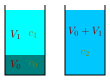
\includegraphics[width = 0.5\textwidth]{mixing_example}
}
\end{tabular}
If we know the volumes \(V_0\) and \(V_1\), and the concentrations \(c_0\) and \(c_1\), and are interested in the final concentration \(c_2\), the above equation can be solved to yield: 
\[c_0 \cdot V_0 + c_1 \cdot V_1 = c_2(V_0 + V_1) \iff c_2 = \frac{c_0 \cdot V_0 + c_1 \cdot V_1}{V_0 + V_1}\]
If we know volume \(V_0\) and concentrations \(c_0\) and \(c_1\), but are instead interested in finding the volume \(V_1\) needed to achieve a target final concentration of \(c_2\), the equation can instead be solved to yield:
\begin{align*}
& c_0 \cdot V_0 + c_1 \cdot V_1 = c_2(V_0 + V_1) \\
\iff & c_0 \cdot V_0 + c_1 \cdot V_1 = c_2 \cdot V_0 + c_2 \cdot V_1 \\
\iff & (c_2 - c_1)V_1 = (c_0 - c_2)V_0 \\
\iff & V_1 = \frac{c_0 - c_2}{c_2 - c_1}V_0
\end{align*}

\vspace{5mm}

If \(V_0 = 3.5\text{L}\); \(V_1 = 2.5\text{L}\); \(c_0 = 0.1\text{g/mL}\); \(c_1 = 0.01\text{g/mL}\); then to compute \(c_2\) we must first standardize the units: Replace \(\text{g/mL}\) with \(\frac{\text{g}}{10^{-3}L} = 10^3\text{g/L}\), or replace \(\text{L}\) with \(10^3\text{mL}\). It is simpler to replace \(\text{L}\) with \(10^3\text{mL}\), so volume is measured in \(\text{mL}\)'s, and concentration is measured in \(\text{g/mL}\). Hence

\[V_0 = 3.500 \times 10^3\text{mL} \;;\; V_1 = 2.500 \times 10^3\text{mL} \;;\; c_0 = 1.000 \times 10^{-1}\text{g/mL} \;;\; c_1 = 1.000 \times 10^{-2}\text{g/mL}\]

\begin{align*}
c_2 = & \frac{c_0 \cdot V_0 + c_1 \cdot V_1}{V_0 + V_1} 
= \frac{(3.500 \times 10^2\text{g}) + (2.500 \times 10^1\text{g})}{6.000 \times 10^3\text{mL}} 
= \frac{3.750 \times 10^2\text{g}}{6.000 \times 10^3\text{mL}} 
\approx 6.250 \times 10^{-2}\text{g/mL} \\
= & 0.06250 \text{g/mL}
\end{align*}

\vspace{5mm}

If \(V_0 = 3.5\text{L}\); \(c_0 = 0.1\text{g/mL}\); \(c_1 = 0.01\text{g/mL}\); and \(c_2 = 0.05\text{g/mL}\); then to compute \(V_1\) we must first standardize the units: replace \(\text{L}\) with \(10^3\text{mL}\), so volume is measured in \(\text{mL}\)'s, and concentration is measured in \(\text{g/mL}\). Hence 

\[V_0 = 3.500 \times 10^3\text{mL} \;;\; c_0 = 1.000 \times 10^{-1}\text{g/mL} \;;\; c_1 = 1.000 \times 10^{-2}\text{g/mL} \;;\; c_2 = 5.000 \times 10^{-2}\text{g/mL}\]

\begin{align*}
V_1 = & \frac{c_0 - c_2}{c_2 - c_1}V_0
= \frac{5.000 \times 10^{-2}\text{g/mL}}{4.000 \times 10^{-2}\text{g/mL}} (3.500 \times 10^3\text{mL})
= (1.250)(3.500 \times 10^3\text{mL}) 
\approx 4.375 \times 10^3\text{mL} \\
= & 4.375 \text{L}
\end{align*}




%\section*{Exact values vs approximations}




\end{document}















